\documentclass[a4paper]{article} 
\addtolength{\hoffset}{-2.25cm}
\addtolength{\textwidth}{4.5cm}
\addtolength{\voffset}{-3.25cm}
\addtolength{\textheight}{5cm}
\setlength{\parskip}{0pt}
\setlength{\parindent}{0in}

\usepackage{natbib}
\usepackage{blindtext} % Package to generate dummy text
\usepackage{charter} % Use the Charter font
% \usepackage[utf8]{inputenc} % Use UTF-8 encoding
\usepackage{microtype} % Slightly tweak font spacing for aesthetics
\usepackage{amsthm, amsmath, amssymb} % Mathematical typesetting
\usepackage{float} % Improved interface for floating objects
\usepackage{hyperref} % For hyperlinks in the PDF
\usepackage{graphicx, multicol, multirow} % Enhanced support for graphics
\usepackage{xcolor} % Driver-independent color extensions
\usepackage{pseudocode} % Environment for specifying algorithms in a natural way
\usepackage[ddmmyyyy]{datetime} % Uses YEAR-MONTH-DAY format for dates
%\usepackage{gensymb}
\usepackage{bibentry}
\usepackage{color}
\usepackage{booktabs}
\usepackage{enumitem}
\usepackage{tikz}
\usepackage{psfrag}
\usepackage{forest}
\usepackage{makecell}
\usepackage{adjustbox}
\usepackage{xeCJK}
% \setCJKmainfont{Noto Serif CJK SC}
% \setCJKmonofont{Noto Sans Mono CJK SC}
\setCJKmainfont{SimSun}
\setCJKmonofont{SimSun-ExtB}

\usepackage{fancyhdr} % Headers and footers
\pagestyle{fancy} % All pages have headers and footers
\fancyhead{}\renewcommand{\headrulewidth}{0pt} % Blank out the default header
\fancyfoot[L]{} % Custom footer text
\fancyfoot[C]{} % Custom footer text
\fancyfoot[R]{\thepage} % Custom footer text
\newcommand{\note}[1]{\marginpar{\scriptsize \textcolor{red}{#1}}} % Enables comments in red on margin

\renewenvironment{abstract}{\vskip.075in\centerline{\textbf{\large
ABSTRACT}}\vspace{0.5ex}\begin{quote}}{\par\end{quote}\vskip 1ex}

\hypersetup{
    colorlinks=true,
    linkcolor=red,
    citecolor=cyan,
    filecolor=magenta,      
    urlcolor=magenta,
    }

%----------------------------------------------------------------------------------------

\usepackage{indentfirst}
\setlength{\parindent}{2em}
\usepackage{caption}
\usepackage{subcaption}
\usepackage{hyperref}
%-------------------------------
%	TITLE VARIABLES (identify your work!)
%-------------------------------

\newcommand{\yourname}{向楚阳} % replace with your name
\newcommand{\yournetid}{kroxxcy777} % replace with your NetID
\newcommand{\youremail}{kroxxcy777@sjtu.edu.cn} % replace with your email
\newcommand{\papertitle}{AIH4CO: AI-Assisted Heuristics to Solve Combinatorial Optimization Problems} % replace with paper title
\newcommand{\authorship}{Chuyang Xiang} % replace with your English name

\begin{document}

%-------------------------------
%	TITLE SECTION (do not modify unless you really need to)
%-------------------------------
\fancyhead[C]{}
\hrule \medskip
\begin{minipage}{0.295\textwidth} 
\raggedright
% \footnotesize
% \normalsizeyourname
\textbf{\textcolor{blue}{\yourname \hfill\\ 
\yournetid \hfill\\ }
\youremail}
\end{minipage}
\begin{minipage}{0.69\textwidth} 
\centering 
\Large
\textbf{\papertitle}\\ 
\normalsize 
\authorship
\end{minipage}
\medskip\hrule 
\bigskip


\begin{abstract}
Combinatorial optimization problems are addressed on a daily basis. Nevertheless, optimal solutions remain challenging to find. In recent years, researchers have sought to enhance traditional heuristic techniques through the incorporation of AI methodologies, thereby proposing novel approaches to the delivery of optimal or near-optimal solutions. However, there is currently no up-to-date review of this field. The objective of this survey is to fill this gap in order to stimulate new ideas on this combination. Firstly, the key concepts are explained. Then, the collected methods are categorised based on a proposed taxonomy, and some analysis of current challenges is provided. Finally, promising future research directions are proposed. Relevant papers up-to-date in this field can be found via the following link: \url{https://github.com/KROX777/Awesome-AIH4CO}.
\end{abstract}

\section{Introduction} % this is an example
Combinatorial optimization problems (COP) form the foundation of numerous practical problems in real-life scenario such as vehicle routing and scheduling, electronic design automation, resource allocation, etc. These problems typically aim to minimize a specific cost function within discrete structures, often under \textit{complex constraints}. Since they're often NP-Hard problems \citep{Karp}, loads of heuristic \citep{Boussaïd,Farhi} algorithms are developed to offer more cost-efficient solutions. In the past decade, as AI-driven methods are becoming ubiquitous, methods like Machine learning (ML), Graph Neural Networks (GNN), Reinforcement Learning (RL), etc. have emerged as state-of-the-art techniques in CO problem-solving while still having room for improvement. On the other hand, researchers are also trying to utilize modern AI methods to refresh traditional heuristics given the superiority of well-established, highly optimized heuristics over ML, RL methods. \citep{darvariu}

However, while research on integrating AI with heuristics for CO (AIH4CO) has increased, comprehensive and systematic surveys specifically focusing on this integration are limited. Lots of surveys have been done on CO problem-solving, but only cover one method in isolation \citep{Boussaïd,Quentin} or the multiple solutions to one specific COP \citep{Zhang}. \citet{Talbi} have explored how researchers have combined ML and heuristics to solve general optimization problems. \citet{Maryam,dosSantos2014} have done surveys on similar topics but fail to be up-to-date, only including the integration of heuristics and traditional ML algorithms. 

The major contributions of this survey lie in three main aspects:
\begin{enumerate}
    \item {\textbf{Up-to-date overview:}} The survey provides a focused overview on the work to-date on AIH4CO, addressing the gap mentioned above.
    \item {\textbf{Taxonomy optimization:}} The survey updates the taxonomy proposed by \citet{Maryam} and \citet{Talbi} to better conclude recent models and guide future research.
    \item {\textbf{Re-evalution of recent ideas:}} The survey collates novel benchmark methods for several COPs and re-evaluates the value of several models.
\end{enumerate}

\section{Preliminaries}
\subsection{Combinatorial Optimization Problems (COP)}
As mentioned above, COPs are a family of problems aiming to minimize a specific cost function within discrete structures under complex constraints. Here we listed some representative COPs. Additionally, we denote an undirected and weighted graph \( G = (V, E) \).
\begin{enumerate}
% \item {\textbf{Graph Matching:}} This refers to establishing node correspondences between two or among multiple graphs. For the classic setting of two-graph matching between graphs $G1$, $G2$, the problem can be written by the general quadratic assignment programming (QAP) problem:
% \[
% J(\mathbf{X}) = vec(\mathbf{X})^T\mathbf{K}vec(\mathbf{X})
% \]
% \[
% \mathbf{X} \in \{0,1\}^{N \times N}, \quad \mathbf{X} \mathbf{1} = \mathbf{1}, \quad \mathbf{X}^{\top} \mathbf{1} \leq \mathbf{1}
% \]
\item {\textbf{Traveling Salesman Problem (TSP):}} Given a set of \( n \) cities represented as vertices \( V = \{1, 2, \ldots, n\} \) and a distance matrix \( D = (d_{ij}) \) where \( d_{ij} \) is the distance between city \( i \) and city \( j \), the goal is to find a permutation \( \pi \) of \( V \) that minimizes the total tour length:
\[
\min_{\pi} \sum_{i=1}^{n} d_{\pi(i) \pi(i+1)},
\]
where \( \pi(n+1) = \pi(1) \) to ensure the tour returns to the starting city.
\item {\textbf{Maximum Cut Problem  (MCP):}} The goal is to find a partition of the vertex set \( V = S \bigsqcup T \) that maximizes the number of edges between \( S \) and \( T \), i.e., \( \left| \left\{ \{v_i, v_j\} \in E : v_i \in S, v_j \in T \right\} \right| \)
\item {\textbf{Minimum Dominating Clique Problem (MDCP):}} The goal is to find the smallest possible subset \( S \) of \( V \) such that \( S \) is a clique and dominates \( V \setminus S \), i.e., \( \forall u \in V \setminus S \), \( \exists v \in S \) such that \( \{v, u\} \in E \). 
\item {\textbf{Maximum Minimal Cut Problem (MMCP):}} The goal is to find a partition of the vertex set \( V \) into two disjoint subsets \( V_1 \) and \( V_2 \) such that the minimum cut between \( V_1 \) and \( V_2 \) is maximized.
\item{\textbf{Maximum Independent Set Problem (MISP):}} The goal is to find the largest possible subset of vertices \( S \subseteq V \) such that no two vertices in \( S \) are adjacent (i.e., for any \( u, v \in S \), \( \{u, v\} \notin E \)).
\item{\textbf{Mixed Integer Programming (MIP):}} The goal is to optimize a linear objective function subject to linear constraints, with some variables constrained to be integers. Formally:
\[
\min_{x, y} \, c^T x + d^T y
\]
subject to
\[
A x + B y \leq b,
\]
where \( x \in \mathbb{Z}^p \) (integer variables), \( y \in \mathbb{R}^q \) (continuous variables), and \( A \), \( B \), \( c \), \( d \), and \( b \) are matrices and vectors of appropriate dimensions.

\end{enumerate}

Only a few problems are listed. For more problem descriptions, please refer to \citet{Maryam}.

\subsection{Meta-Heuristics (MH)}
Meta-Heuristics is a broad concept encompassing all high-level heuristic algorithms designed to find near-optimal solutions across a wide range of COPs. Different from ML, which utilizes data-driven, generalizable approaches that learn patterns , MH are simpler, rule-based methods designed for specific tasks, thus providing acceptable solutions in reasonable computational time \citep{Hertz}. Typical MH algorithms include Simulated Annealing (SA), Tabu Search (TS), Ant Colony Optimization (ACO), etc. They are primarily dedicated to directly solving problems. However, they often require manually designed and tuned strategies, making them less robust in front of new situations.

\subsection{Hyper-Heuristics (HH)}
Different from MH, HH is a kind of search techniques that can generate solutions for a wide range of problem domains instead of using specific technique to each problem instance thanks to the fact that HH works in the heuristic search space instead of a solution space \citep{Ahmed}. Fig.~\ref{fig:hyper_heuristic} below presents two forms of HH \citep{Edmund}. Given this advantage, HH already has remarkable performance in certain CO problems and presents a higher level of generality \citep{Gabriel}. However, they are still limited by the heuristic space predefined by human experts, calling for AI-driven models to automate this process \citep{Ye}.
\begin{figure}[h]
\centering
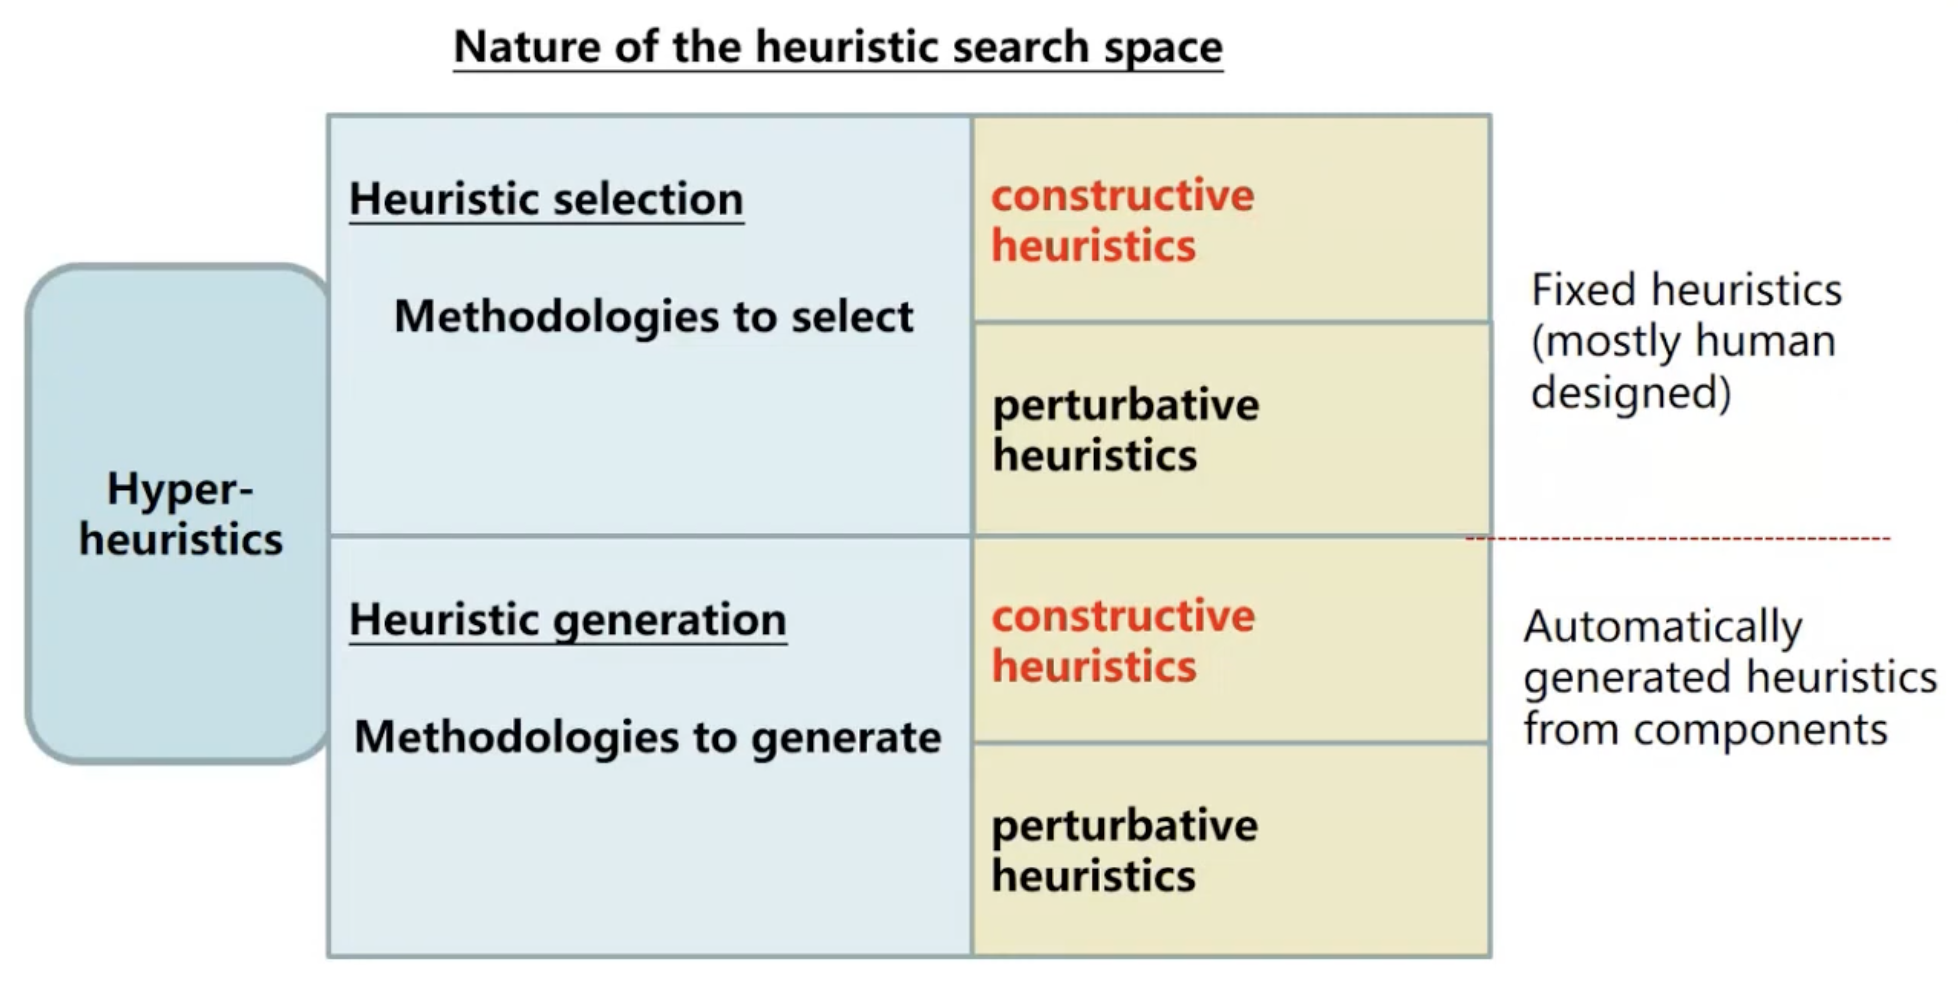
\includegraphics[width=0.5\textwidth]{figures/Hyper Heuristic.png}
    \caption{\label{fig:hyper_heuristic}The Classification of Hyper-Heuristic}
\end{figure}

% \subsection{Neural Combinatorial Optimization (NCO)}
% This is a well-surveyed strategy \citep{Quentin} which refers to learning the problem directly using ML-based, RL-based or GNN-based methods. This can be regarded as an alternative form of Hyper-Heuristics, wherein neural architectures and solution pipelines define a heuristic space, and training algorithms search within it \citep{Ye}.

\section{AIH4CO Techniques and their Analysis}
This survey restructured the taxonomy method for how AI is used in the heuristics that was utilized in \citet{Maryam}  to make it clearer as well as to introduce new ideas like algorithm generation and scheduling. Fig.~\ref{fig:Tax} shows the method. It's noteworthy that the focus of the survey is mainly on \textit{AI-in-Heuristics} and \textit{AI-and-Heuristics}.

\begin{figure}[h]
\centering
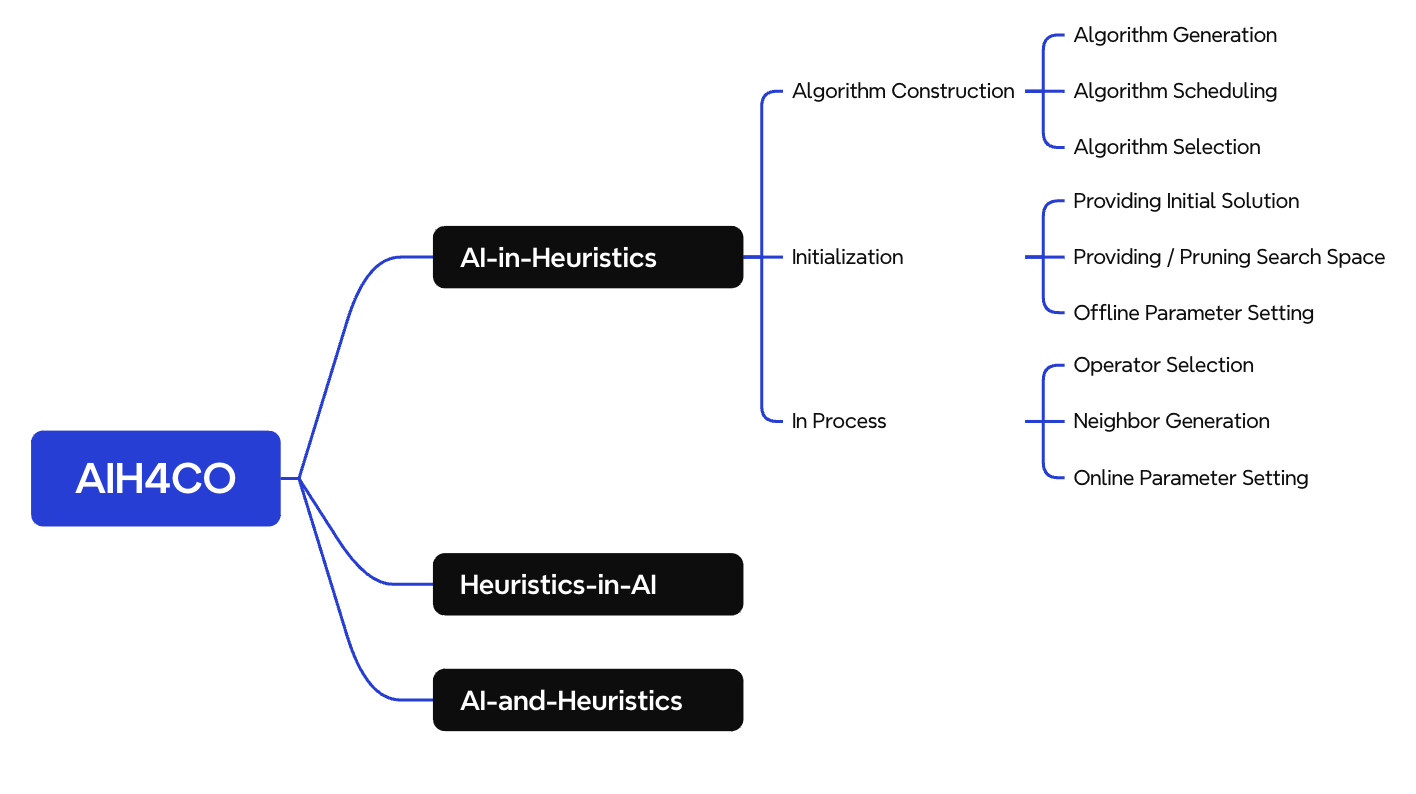
\includegraphics[width=0.8\textwidth]{figures/Taxonomy.png}
    \caption{\label{fig:Tax}Taxonomy of AIH4CO}
\end{figure}

\subsection{AI-in-Heuristics}
\subsubsection{Algorithm Selection \& Generation}
\label{sec:ASG}

Algorithm selection and generation are two major research directions. The former concept is more established, with the Algorithm Search Problem (ASP) having been proposed and researched for a considerable period of time \citep{Maryam} . In comparison, the latter concept gains much development recently with the help of AI. A considerable number of implementations of reinforcement learning (RL) on CO problems have adopted the concept of algorithm generation \citep{Nina}. However, pure RL is beyond the scope of this survey. The present survey focuses on RL for heuristics and heuristic generation HH as major methods in algorithm generation. Fig ~\ref{fig:rl_ag} illustrates how RL can be used for heuristics generation \citep{Haoran}. This survey presents recent research employing HH, as well as the conventional ASP-oriented meta-learning approach, as illustrated in Table~\ref{tab:AS}.

\begin{figure}[h]
\centering
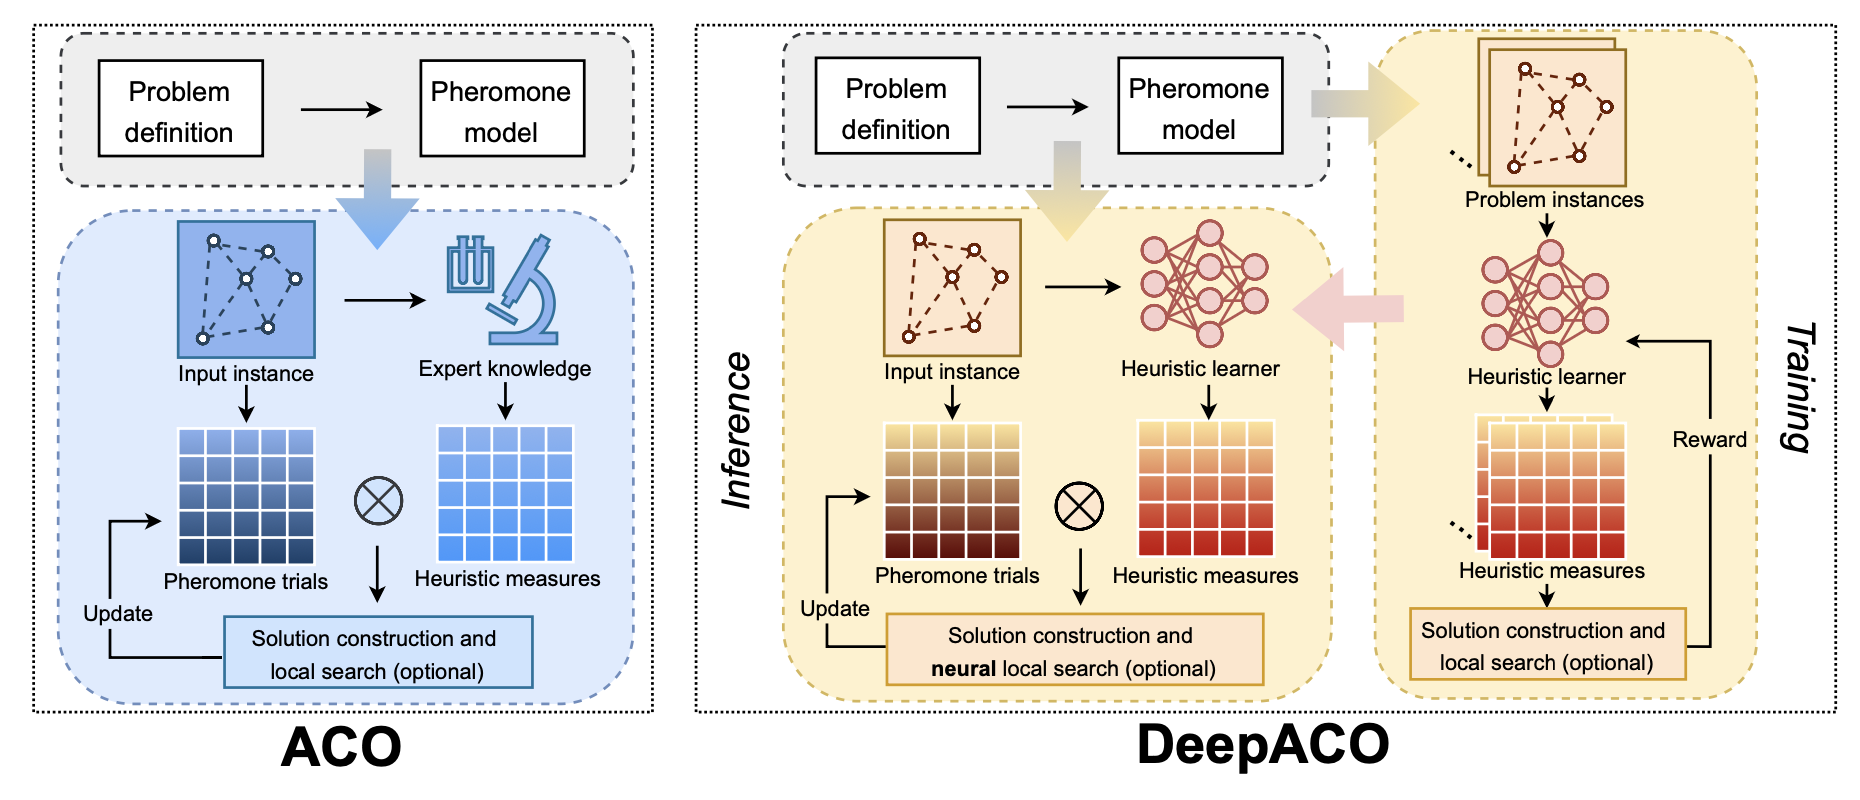
\includegraphics[width=0.8\textwidth]{figures/RL for Algorithm Generation.png}
    \caption{\label{fig:rl_ag}RL for Heuristics Generation}
\end{figure}

The approach of heuristic generation often stands out as it does not necessitate the prior construction of manually crafted algorithms.  \citep{Edmund} This makes heuristic generation HH more general and robust. Nevertheless, when a substantial number of well-designed candidate algorithms are available, meta-learning and heuristic selection HH are optimal choices thanks to their better performance and low computational costs.

It is noteworthy that GNNs have emerged as a prevalent tool for learning algorithmic tasks, which are a crucial aspect of both algorithm selection and generation \citep{Khalil,Shen}. However, \citet{Ankur} proposed a benchmark standard and put forward the notion that GNNs do not actually perform as well as it's expected since linear regression even outperforms GNNs in some highly cited models \citep{Khalil}, which is alarming and disappointing. The notion corresponded with what \citet{Angelini} has expressed.

\begin{table}[h]
\centering
\caption{Methods on algorithm selection \& generation}\label{tab:AS}
\resizebox{1\textwidth}{!}{
\begin{tabular}{cccccc}
\multicolumn{1}{c}{\bf Method} &\multicolumn{1}{c}{\bf Heuristic Strategy}  &\multicolumn{1}{c}{\bf AI Model} &\multicolumn{1}{c}{\bf CO Problems}  &\multicolumn{1}{c}{\bf Additional Techniques}  &\multicolumn{1}{c}{\bf Selection or Generation}
\\ \hline \\
\citet{Khalil} &Forward Greedy   &RL,GNN  &COP over graphs &/ &Generation\\
\citet{Rosa}   &MH  &Linear Regression &CB-CTT &Meta-learning Framework &Selection\\
\citet{Shen}       &MH  &GCN   &MIP &PB-DFS &Selection\\
\citet{Haoran} &MH(ACO) &DRL  &General &Local Search &Generation\\
\citet{Romera} &HH  &LLM  &General  &Evolutionary Framework &Both\\
\citet{Ye}     &HH,GLS   &LLM    &General   &Gene Language Hyper-Herusitic &Both\\
\citet{Liu}    &HH    &LLM    &General   &Evolutionary Computation(EC) &Both\\
\end{tabular}
}
\end{table}

\subsubsection{Algorithm Scheduling}
Algorithm scheduling refers to utilizing AI methods to decide which heuristics to run and/or for how long \citep{Scavuzzo}. This is similar to one function of heuristic selection HH. Two advantages can be identified. The first is the combination of different heuristics to achieve optimal performance. The second is the ability to exert greater control over the computational budget. The process is illustrated in Fig ~\ref{fig:HS}, and the techniques are listed below on Table ~\ref{tab:AS}.

\begin{figure}[h]
\centering
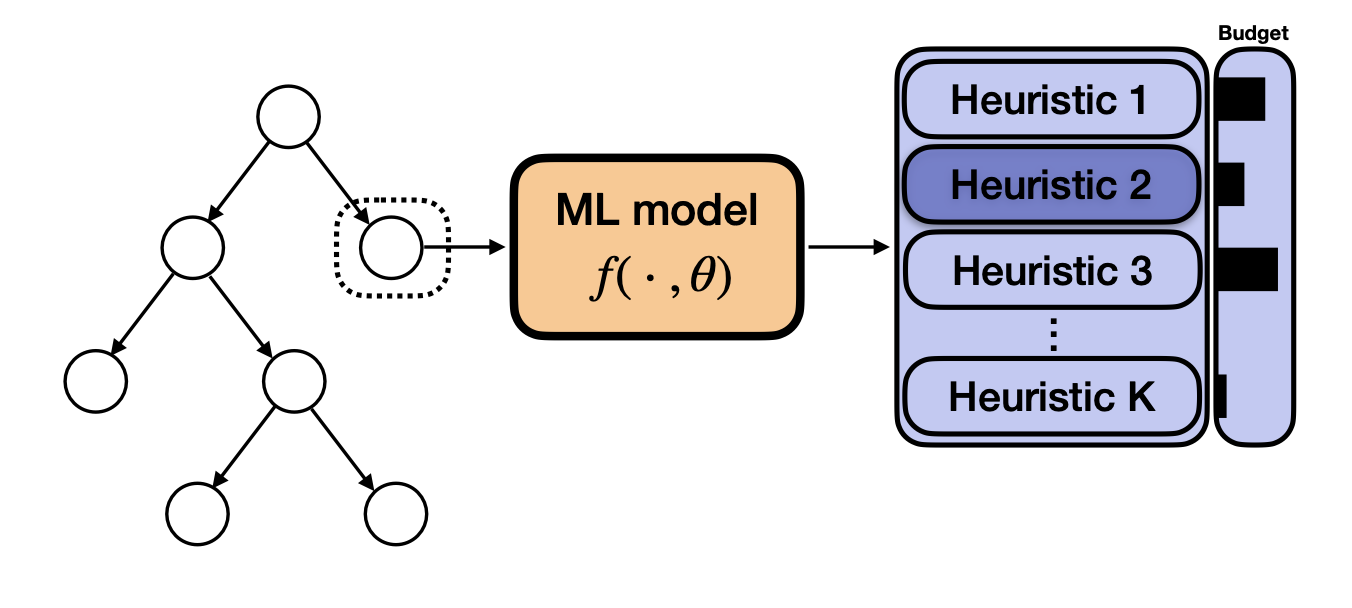
\includegraphics[width=0.5\textwidth]{figures/Heuristics Scheduling.png}
    \caption{\label{fig:HS}Heuristics Scheduling}
\end{figure}

\begin{table}[h]
\centering
\caption{Methods on algorithm scheduling}\label{tab:AS}
\resizebox{1\textwidth}{!}{
\begin{tabular}{cccccc}
\multicolumn{1}{c}{\bf Method} &\multicolumn{1}{c}{\bf Heuristic Strategy}  &\multicolumn{1}{c}{\bf AI Model} &\multicolumn{1}{c}{\bf CO Problems}  &\multicolumn{1}{c}{\bf Additional Techniques}
\\ \hline \\
\citet{Khalil2} &B\&B   &Logistic Regression  &MIP &/ \\
\citet{Chmiela2} &B\&B,LNS,Diving    &ML   &MIP  &/ \\
\citet{Chmiela}        &B\&B,LNS,Diving    &ML   &MIP   &$\epsilon$-greedy bandit algorithm
\end{tabular}
}
\end{table}

\subsubsection{Initialization}

Any heuristics starts its search process from an initial solution or a population of solutions \citep{Maryam}. Fortunately, it's easy for machine learning to identify elements to either be or not to be in the optimal solution based on available information \citep{Juho}. So the AI-based initialization can provide good initial solutions \citep{Jiwei}, provide search space or prune search space \citep{Xin,Congsong,Juho,Jiwei} through learning. Initial parameters, which are essential to MH, can also be learned. Concrete methods comparison are given below on Table~\ref{tab:INI}.

Initialization has long been shown to be the single most impactful component of CO solvers \citep{Achterberg}, making it a promising research direction. Among these reviewed essays, \citet{Juho} stands out for its unique self-designed heuristics ALTHEA, which combines exact algorithms with light-weighted machine learning methods to prune search space.

\begin{table}[h]
\centering
\caption{Methods on initialization}\label{tab:INI}
\resizebox{1\textwidth}{!}{
\begin{tabular}{ccccc}
\multicolumn{1}{c}{\bf Method} &\multicolumn{1}{c}{\bf Heuristic Strategy}  &\multicolumn{1}{c}{\bf AI Model} &\multicolumn{1}{c}{\bf CO Problems}  &\multicolumn{1}{c}{\bf Additional Techniques}
\\ \hline \\
\citet{Zhuwen}         &Branching Heuristic &GNN   &MISP &/\\
\citet{Xin}         &LKH  &SGN  &TSP &/\\
\citet{Juho}        &Self-Designed &Gradient Boosted Trees  &General &Chi-square
Statistics\\
\citet{Congsong}       &Branching Heuristic &GNN   &MDCP &/\\
\citet{Huaiyuan}   &Heuristic Tree Transformation   &GNN   &MMCP &Relaxation-plus-Rounding\\
\citet{Jiwei}       &Local Search    &SVM       &Steiner Tree Problem    &/
\end{tabular}
}
\end{table}

\subsubsection{In Process}
AI methods can also help heuristics either decide upon the selection of operators at each step of the search process based on the status of the search and the operators' performance history \citep{Karimi2} or identify the common characteristics that are often present in effective solutions and use this knowledge to generate new solutions with the same characteristics by fixing specific solution characteristics \citep{Fairee, Huang}. On the other hand, many heuristics rely heavily on online parameter setting, which can also be done by AI methods \citep{Oztop}. Here are some implementations on Table ~\ref{tab:IP}.

Generalization is the hugest challenge in this area given the need of executing (extremely) fast primal heuristics in process \citep{Scavuzzo}.

\begin{table}[h]
\centering
\caption{Methods in process}\label{tab:IP}
\resizebox{1\textwidth}{!}{
\begin{tabular}{ccccc}
\multicolumn{1}{c}{\bf Method} &\multicolumn{1}{c}{\bf Heuristic Strategy}  &\multicolumn{1}{c}{\bf AI Model} &\multicolumn{1}{c}{\bf CO Problems}  &\multicolumn{1}{c}{\bf Additional Techniques}
\\ \hline \\
\citet{Benlic}   &Breakout Local Search &RL  &Vertex separator problem &/ \\
\citet{Fairee}    &Artificial Bee Colony Optimization   &RL     &TSP &/ \\
\citet{Mosadegh}    &MH(SA)  &RL  &Assembly line sequencing &/ \\
\citet{Oztop}        &MH(Variable Neighborhood Search) &RL &Flowshop scheduling problem &/ \\
\citet{Karimi2} &MH(Iterated Greedy) &RL(Q-Learning) &Permutation flowshop scheduling &/ \\
\citet{Tonshoff}    &Local Search &GNN, RL  &MCP &/ \\
\citet{Huang}   &LNS    &Contrastive Learning (CL) &MIP &Graph Attention Networks \\
\end{tabular}
}
\end{table}


\subsection{AI-and-Heuristics}
Here, heuristics and AI methods perform their own functions independently to solve CO problems. These efforts are listed on Table \ref{tab:CP}.

\begin{table}[h]
\centering
\caption{Methods on AI-and-Heuristics}\label{tab:CP}
\resizebox{0.8\textwidth}{!}{
\begin{tabular}{ccccp{6cm}}
\multicolumn{1}{c}{\bf Method} &\multicolumn{1}{c}{\bf Heuristic Strategy}  &\multicolumn{1}{c}{\bf AI Model} &\multicolumn{1}{c}{\bf CO Problems}  &\multicolumn{1}{c}{\bf How they Cooperate}
\\ \hline \\
\citet{Karimi}      &Iterated Local Search  &K-Means &IPP &K-Means to link multi-objective population-based MHs with
single-solution based MHs\\
\citet{Hou}         &MH  &Transformer  &VRP &Transformer to divide VRPs into sub-VRPs and MH to solve sub-VRPs
\end{tabular}
}
\end{table}

\section{Novel Benchmark Standards}
The survey also gathers some novel benchmark standards to help evaluate future work. \citet{Lu} designed RL-based attacker and proposed a general framework for evaluating robustness of CO solvers on graphs. More specifically, \citet{Angelini} put forward some hard benchmarks on MCP and MISP and \citet{Ankur} also proposed a strict benchmark for MCP in terms of three dimensions: objective value, generalization, and scalability.

\section{Conclusions \& Outlooks}
The survey looks at multiple ways that heuristics can be combined with AI methods to solve CO problems. With regard to the future research directions, \citet{Maryam} has proposed utilizing clustering ML methods to pre-process data and using AI for multiple purposes with most models proposed so far focusing on specific aspects of heuristic processes, which still applies to the present. In addition to them, other five future research directions are provided based on the findings:

\begin{enumerate}
    \item{\textbf{Make Full Use of LLM:}} As LLM begins to support code generation and optimisation, new avenues for research on this topic emerge. Research such as \citet{Ye} remains constrained by a relatively naive idea. The field is in need of more ambitious approaches that leverage LLM and heuristics to solve CO problems.
    \item{\textbf{Towards Interpretable AI:}} CO problems are calling for more interpretable methods. The recently-proposed Kolmogorov-Arnold Network (KAN) \citep{ZLiu} is interpretable to some extent and excels at learning combinatorial structures, which has the potential to be integrated into heuristics and solve CO problems.
    \item{\textbf{AI for Quantum Heuristics:}} The implementation of quantum-related techniques holds considerable promise for the future, with a number of quantum heuristics (such as QAOA) already being developed for use in CO problems \citep{Farhi,Li}. Quantum Neural Network (QNN) was also proposed to solve CO problems \citep{Xinyu}. However, the combination of AI and quantum heuristics remains an area that is yet to be fully explored.
    \item{\textbf{Explore More Out-of-box Combination:}} Most of the works surveyed can be categorized into the four branches AI-in-Heuristics. New combination ideas are too rare in AI-and-Heuristics. Groundbreaking improvements may emanate from completely new ideas.
    \item {\textbf{Unified Benchmark Standards:}} As mentioned in \hyperref[sec:ASG]{Section 3.1.1}, \citet{Ankur} sharply pointed out the significant shortcomings of GNN-assisted heuristics compared with traditional heuristics and linear-regression-assisted ones. This underscored the limitations of benchmark standards employed by researchers.
\end{enumerate}


\bibliographystyle{apalike}
\bibliography{Paper_summaries}
\end{document}

%TODO:
%4. Subtable
%Chang fig2
%\citet{Hendel}       &LNS       &MIP
%how many brnaches? conclusion